\documentclass[11pt]{article}

\usepackage{url}
\usepackage{multicol}
\usepackage[english]{babel}
\usepackage[margin=1in]{geometry}
\usepackage{graphicx}
\usepackage{subcaption}
\usepackage{enumitem}
\usepackage{amsmath}
\usepackage{amssymb}
\usepackage{wasysym}
\usepackage{color}
\usepackage{float}
\usepackage{nomencl}
\usepackage[title]{appendix}
\makenomenclature
\usepackage{pdfpages}
\usepackage{algorithm}
\usepackage{algpseudocode}
\usepackage{hyperref}
\hypersetup{
    colorlinks=true,
    linkcolor=blue,
    filecolor=magenta,      
    urlcolor=cyan,
    pdftitle={Overleaf Example},
    pdfpagemode=FullScreen,
    }
\title{16-745 Optimal Control Lecture 16}
\author{Reid Graves} 

\begin{document}
\maketitle

\section{Last Time}
\begin{itemize}
    \item Optimization with Quaternions
\end{itemize}

\section{Today}
\begin{itemize}
    \item LQR with Quaternions
    \item Quadrotor Control
\end{itemize}

\noindent\rule{\textwidth}{0.4pt} % Horizontal line
\section{LQR with Quaternions}

\begin{itemize}
    \item Naively linearizing a system with a quaternion state results in an uncontrollable linear system
    \item We'll apply our quaternion differentiation tricks to LQR to make this work
    \item Given a reference $\bar{x}_k, \bar{u}_k$ for a discrete time system $f(x_k,u_k):$
    \begin{align*}
        \bar{x}_{k+1} + \Delta x_{k+1} &\approx f(\bar{x}_k + \Delta x_k, \bar{u}_k + \Delta u_k)
        \\
        &\text{First order Taylor expansion:} 
        \\
        &\approx f(\bar{x}_k,\bar{u_k}) + \underbrace{A_k}_{\textcolor{cyan}{\frac{\partial f}{\partial x}}} \Delta x_k + \underbrace{B_k}_{\textcolor{cyan}{\frac{\partial f}{\partial u}}}\Delta u_k
        \\
        \bar{x}_{k+1} &= f(\bar{x}_k,\bar{u_k})\\ 
        \\
        \Delta x_{k+1} &= \underbrace{A_k}_{\textcolor{cyan}{\frac{\partial f}{\partial x}}} \Delta x_k + \underbrace{B_k}_{\textcolor{cyan}{\frac{\partial f}{\partial u}}}\Delta u_k
    \end{align*}
    \item For the quaternion part of the state, we apply the attitude Jacobian to convert $\Delta \rightarrow \phi \in \mathbb{R}^3$:
\begin{align*}
    x &= \begin{bmatrix} r \\ q \\ \theta \\ r \\ \omega \\ \dot{\theta}\end{bmatrix}
    \\
    & \hspace{10mm}r  \quad\textcolor{cyan}{x[1:3]} \\
    & \hspace{10mm}q  \quad\textcolor{cyan}{x[4:7]}\\
    & \hspace{10mm}\theta  \quad\textcolor{cyan}{x[8:n]\text{ (joint angles)}} \\
    & \hspace{12mm} \vdots
\end{align*}
\begin{align*}
    \underbrace{\begin{bmatrix}
        \Delta x_{k+1}[1:3]
        \\
        \phi_{k+1}
        \\
        \Delta x_{k+1}[8:n]
    \end{bmatrix}}_{\textcolor{cyan}{\Delta\tilde{x}_{k+1}}}
    &=
    \underbrace{\begin{bmatrix}
        I & & 0 \\
        & G(\bar{q}_{k+1}) & \\
        0 & & I
    \end{bmatrix}^T}_{\textcolor{cyan}{E(\bar{x}_{k+1})}} A_k
    \underbrace{\begin{bmatrix}
        I & & 0 \\
        & G(\bar{q}_k) & \\
        0 & & I
    \end{bmatrix}}_{\textcolor{cyan}{E{\bar{x}_k}}}
    \begin{bmatrix}
        \Delta x_k[1:3] \\
        \phi_k \\
        \Delta x_k[8:n]
    \end{bmatrix}
    + E^T(\bar{x}_{k+1})B_k\Delta u_k
\end{align*}
Since the B matrix is multiplied by controls, it doesn't need a Jacobian transform on the right. But since it's output is a state, it needs a Jacobian transform on the left.
\item Once we have these ``reduced" Jacobians $\tilde{A}_k, \tilde{B}_k$:
\begin{align*}
    \tilde{A}_k &= E(\bar{x}_{k+1})^TA_kE(\bar{x}_k) & \tilde{B}_k&= E^T(\bar{x}_{k+1})B_k
\end{align*}
We compute the LQR controller as usual.
\item When we run the controller, we calculate $\Delta \tilde{{x}}$ before multiplying by $K$:
\begin{align*}
    \text{given } x_k& & \Delta\tilde{x}_k&= \begin{bmatrix}
        x_k[1:3] - \bar{x}_k[1:3] \\
        \phi(L(\bar{q}_k)^T q_k) \\
        x_k[8:n] - \bar{x}_k[8:n]
    \end{bmatrix}\rightarrow{\textcolor{cyan}{\text{whatever 3 parameter representation you like}}}
    \\
   && u_k &= \bar{u}_k - K_k\Delta\tilde{x}_k
\end{align*}
\end{itemize}

\subsection{Computing error/delta rotations}
\begin{itemize}
    \item Many possible conventions
    \item We will write it as rotation from body frame $B$ to the reference/desired body frame $R$. We want to have the rotation from the body frame to the inertial frame:
    \begin{align*}
        \Rightarrow \underbrace{^NQ^B}_{\textcolor{cyan}{Q}} &= \underbrace{^NQ^R}_{\textcolor{cyan}{\bar{Q}}}\underbrace{^RQ^B}_{\textcolor{cyan}{\Delta Q}} &\Rightarrow \underbrace{(^NQ^R)^{-1}{^NQ^B}}_{\textcolor{cyan}{\bar{Q}^TQ}} &= \underbrace{^RQ^B}_{\textcolor{cyan}{\Delta Q}} 
    \end{align*}
    $Q$ is Inertial frame, $\bar{Q}$ is the frame we want, and $\Delta Q$ is the error
    \item Using quaternions
    \begin{align*}
        \Delta q &= \bar{q}^\dagger * q = L(\bar{q})^Tq
    \end{align*}
\end{itemize}

\section{3D Quadrotor}
\begin{figure}[H]
    \centering
    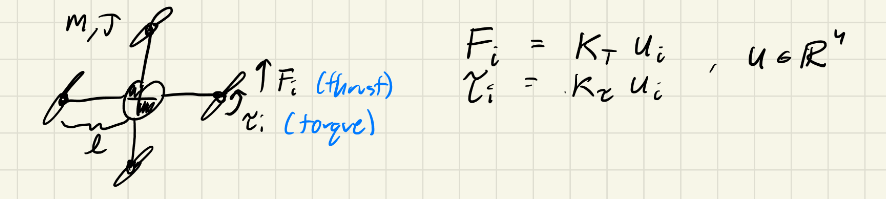
\includegraphics[width=\linewidth]{lecture_16_1.png}
\end{figure}


\begin{itemize}
    \item State:
    \begin{align*}
        x &=
        \begin{bmatrix}
            ^Nr \in \mathbb{R}^3 & \text{Position in } N \text{ frame} \\
            ^Nq^B \in \mathbb{H} & \text{attitude } B\rightarrow N \\
            ^Bv \in\mathbb{R}^3  &\text{linear velocity in } B \text{ frame} \\
            ^B\omega \in\mathbb{R}^3 & \text{angular velocity in } B \text{ frame}
        \end{bmatrix}
    \end{align*}

    \item Kinematics
    \begin{align*}
        ^N\dot{r} &= \ ^Nv = Q \ ^Bv \\
        \dot{q} &= \frac{1}{2}q*\hat{w} = \frac{1}{2}L(q)H \ ^B\omega = \frac{1}{2}G(q)\ ^B\omega
    \end{align*}
    \item Translation Dynamics 
    \begin{align*}
        \underbrace{m \ ^N\dot{v}}_{\textcolor{cyan}{\text{need to rotate into }B \text{ frame}}} &= \ ^NF \leftarrow \textcolor{cyan}{\text{total force}}
        \\
        ^Nv &= Q \ ^Bv \Rightarrow ^N\dot{v} = \underbrace{\dot{Q}}_{\textcolor{cyan}{Q\hat{\omega}}}\ ^Bv + Q\ ^B\dot{v} = Q\hat{\omega} \ ^Bv + Q \ ^B\dot{v} \\
        &\Rightarrow ^B\dot{v} = \overbrace{Q^T\ ^N\dot{v}}^{\textcolor{cyan}{\text{rotate into }B\text{ frame}}} - \underbrace{\ ^B\omega\times \ ^Bv}_ {\textcolor{cyan}{ \text{ extra term from spin}}} \\
        & \Rightarrow ^B\dot{v} = \frac{1}{m} \ ^BF - \ ^B\omega\times \ ^Bv \\
        ^BF &= Q^T\begin{bmatrix}
            0 \\
            0 \\
            -mg
        \end{bmatrix}
        +
        \begin{bmatrix}
            0 & 0 & 0 & 0 \\
            0 & 0 & 0 & 0 \\
            k_T & k_T & k_T & k_T
        \end{bmatrix}
        \begin{bmatrix}
            u_1 \\
            u_2 \\
            u_3 \\
            u_4
        \end{bmatrix}
    \end{align*}
    \item Rotation Dynamics:
    \begin{align*}
        &\underbrace{J \ ^B\dot{\omega} + \ ^ B\omega + \ ^ B\omega\times J \ ^B\omega = \ ^B\tau}_{\textcolor{cyan}{\text{``Eulers equation"}}}
        \\
        &J: \textcolor{cyan}{\text{Inertia matrix}}
        \\
        &\tau :\textcolor{cyan}{\text{total torque}}
        \\
        & ^B\tau = \begin{bmatrix}
            l k_T(u2-u_4) \\
            lk_T(u_3-u_1) \\
            k_\tau(u_1-u_2 + u_3-u_4
        \end{bmatrix}
    \end{align*}
\end{itemize}

\section{Example}
\begin{itemize}
    \item LQR (or convex MPC) with some quaternion tricks is very effective.
\end{itemize}



\end{document}
